\documentclass[11pt,a4paper]{article}
\usepackage[spanish,es-nodecimaldot]{babel}	% Utilizar español
\usepackage[utf8]{inputenc}					% Caracteres UTF-8
\usepackage{graphicx}						% Imagenes
\usepackage[hidelinks]{hyperref}			% Poner enlaces sin marcarlos en rojo
\usepackage{fancyhdr}						% Modificar encabezados y pies de pagina
\usepackage{float}							% Insertar figuras
\usepackage[textwidth=390pt]{geometry}		% Anchura de la pagina
\usepackage[nottoc]{tocbibind}				% Referencias (no incluir num pagina indice en Indice)
\usepackage{enumitem}						% Permitir enumerate con distintos simbolos
\usepackage[T1]{fontenc}					% Usar textsc en sections
\usepackage{amsmath}						% Símbolos matemáticos
\usepackage{listings}
\usepackage{color}

 
\definecolor{codegreen}{rgb}{0,0.6,0}
\definecolor{codegray}{rgb}{0.5,0.5,0.5}
\definecolor{codepurple}{rgb}{0.58,0,0.82}
\definecolor{backcolour}{rgb}{0.99,0.99,0.99}
 
\lstdefinestyle{mystyle}{
    backgroundcolor=\color{backcolour},   
    commentstyle=\color{codegreen},
    keywordstyle=\color{magenta},
    numberstyle=\tiny\color{codegray},
    stringstyle=\color{codepurple},
    basicstyle=\footnotesize,
    breakatwhitespace=false,         
    breaklines=true,                 
    captionpos=b,                    
    keepspaces=true,                 
    numbers=left,                    
    numbersep=5pt,                  
    showspaces=false,                
    showstringspaces=false,
    showtabs=false,                  
    tabsize=2
}
 
\lstset{style=mystyle, language=Python}

% Comando para poner el nombre de la asignatura
\newcommand{\asignatura}{Inteligencia de Negocio}
\newcommand{\autor}{José María Sánchez Guerrero}
\newcommand{\titulo}{Práctica 2}
\newcommand{\subtitulo}{Visualización y segmentación}

% Configuracion de encabezados y pies de pagina
\pagestyle{fancy}
\lhead{\autor{}}
\rhead{\asignatura{}}
\lfoot{Grado en Ingeniería Informática}
\cfoot{}
\rfoot{\thepage}
\renewcommand{\headrulewidth}{0.4pt}		% Linea cabeza de pagina
\renewcommand{\footrulewidth}{0.4pt}		% Linea pie de pagina

\begin{document}
\pagenumbering{gobble}

% Pagina de titulo
\begin{titlepage}

\begin{minipage}{\textwidth}

\centering

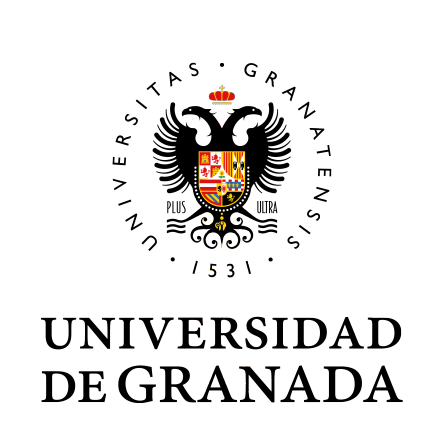
\includegraphics[scale=0.5]{img/ugr.png}\\

\textsc{\Large \asignatura{}\\[0.2cm]}
\textsc{GRADO EN INGENIERÍA INFORMÁTICA}\\[1cm]

\noindent\rule[-1ex]{\textwidth}{1pt}\\[1.5ex]
\textsc{{\Huge \titulo\\[0.5ex]}}
\textsc{{\Large \subtitulo\\}}
\noindent\rule[-1ex]{\textwidth}{2pt}\\[3.5ex]

\end{minipage}

\vspace{0.5cm}

\begin{minipage}{\textwidth}

\centering

\textbf{Autor}\\ {\autor{}}\\[2.5ex]
\textbf{Rama}\\ {Sistemas de Información}\\[2.5ex]
\vspace{0.3cm}


\includegraphics[scale=0.3]{img/etsiit.jpeg}

\vspace{0.3cm}
\textsc{Escuela Técnica Superior de Ingenierías Informática y de Telecomunicación}\\
\vspace{1cm}
\textsc{Curso 2020-2021}
\end{minipage}
\end{titlepage}

\pagenumbering{arabic}
\tableofcontents
\thispagestyle{empty}				% No usar estilo en la pagina de indice

\newpage

\setlength{\parskip}{1em}



\section{Visualización}

Partiendo del dataset de mamografías de la práctica anterior, tendremos que realizar distintas visualizaciones y analizar los
datos que tenemos para cada uno de los preprocesamientos. En mi caso, yo ya mostré en mi práctica anterior una pequeña visualización
de los datos (y que los volveré a mostra para analizarlos mejor), pero en esta completaremos más detalladamente la información.

\subsection{Visualización de las medidas}

Lo primero que pudimos observar, es que tenemos tanto datos numéricos, como datos categóricos. También vimos que hay varias celdas
con datos erróneos o perdidos (representados con el valor $NaN$):

\begin{table}[H]
    \centering
    \resizebox{325px}{!}{%
    \begin{tabular}{|c|c|c|c|c|c|c|}
    \hline
    \textbf{} & \textbf{BI-RADS} & \textbf{Age} & \textbf{Shape} & \textbf{Margin} & \textbf{Density} & \textbf{Severity} \\ \hline
    \textbf{0} & 5.0 & 67.0 & L & 5.0 & 3.0 & maligno \\ \hline
    \textbf{1} & 4.0 & 43.0 & R & 1.0 & NaN & maligno \\ \hline
    \textbf{2} & 5.0 & 58.0 & I & 5.0 & 3.0 & maligno \\ \hline
    \textbf{3} & 4.0 & 28.0 & R & 1.0 & 3.0 & benigno \\ \hline
    \textbf{4} & 5.0 & 74.0 & R & 5.0 & NaN & maligno \\ \hline
    \end{tabular}%
    }
\end{table}

Debido a esto, es importante procesarlos para que nuestros algoritmos funcionen correctamente. La técnica que elegimos en la práctica
anterior fue simplemente la de eliminar estos datos erróneos, con el siguiente resultado:

\begin{figure}[H]
    \centering
    
    \begin{minipage}{0.5\textwidth}
        \centering
        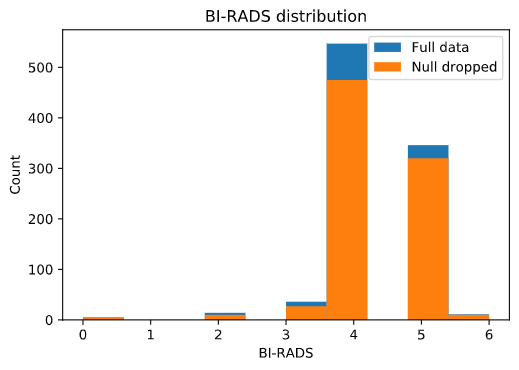
\includegraphics[scale=0.35]{img/birads-distribution.png}
    \end{minipage}%
    \begin{minipage}{0.5\textwidth}
        \centering
        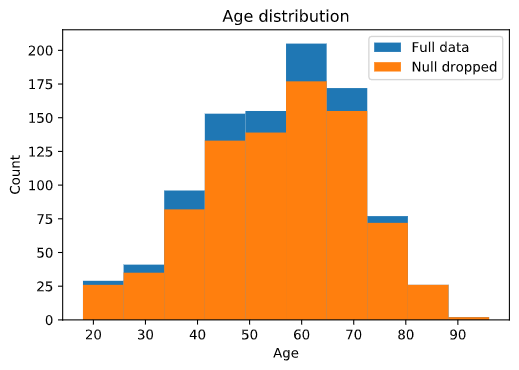
\includegraphics[scale=0.35]{img/age-distribution.png}
    \end{minipage}
    
\end{figure}
    
    
\begin{figure}[H]
    \centering
    
    \begin{minipage}{0.5\textwidth}
        \centering
        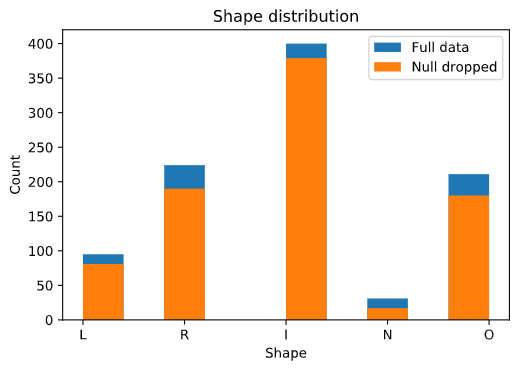
\includegraphics[scale=0.35]{img/shape-distribution.png}
    \end{minipage}%
    \begin{minipage}{0.5\textwidth}
        \centering
        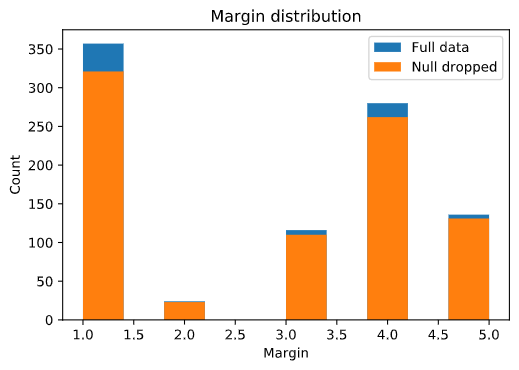
\includegraphics[scale=0.35]{img/margin-distribution.png}
    \end{minipage}
    
\end{figure}
    
    
\begin{figure}[H]
    \centering
    
    \begin{minipage}{0.5\textwidth}
        \centering
        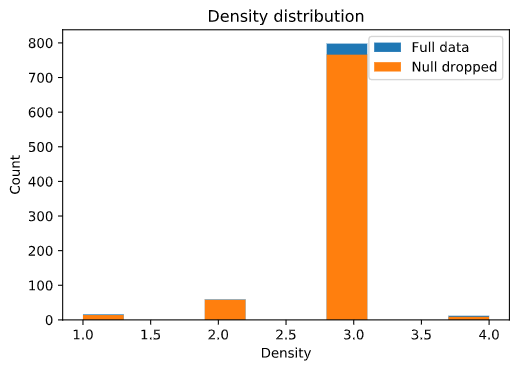
\includegraphics[scale=0.35]{img/density-distribution.png}
    \end{minipage}%
    \begin{minipage}{0.5\textwidth}
        \centering
        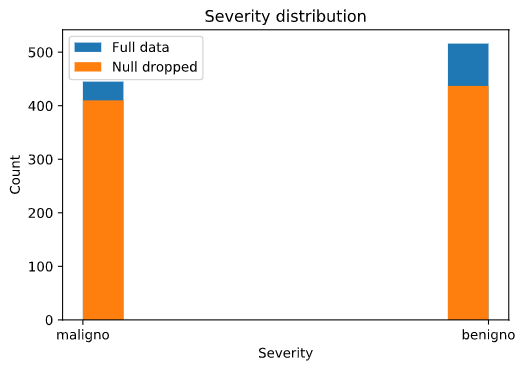
\includegraphics[scale=0.35]{img/severity-distribution.png}
    \end{minipage}
    
\end{figure}
    
Otra estrategia de preprocesamiento que podríamos haber utilizado es la de completar esos valores con datos. Esto a veces puede
no tener sentido, ya que en algunos atributos, como por ejemplo la edad, no vas a asignarle a todos los datos que faltan el valor
de 0 años. Para estos casos veremos otra solución más adelante.

Sin embargo, tenemos atributos como la forma (''\textit{Shape}''), que ya de por sí tienen un valor ''No definido'' con varios
datos en él. Gracias a esto, los datos erróneos o nulos del dataset los podemos meter en esta categoría. 
\begin{figure}[H]
    \centering
    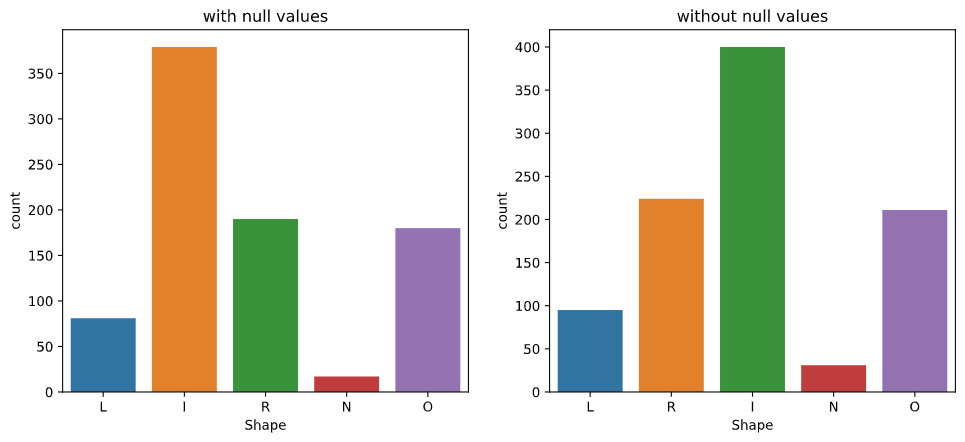
\includegraphics[scale=0.35]{img/shape-refill.png}
\end{figure}

\newpage

¿Qué estrategia diferente podemos utilizar entonces para el resto sin eliminarlos ni poner valores sin sentido? Tenemos varias
opciones. La primera que se nos viene a la cabeza es hacer la media la media entre todos los parámetros y devolver su resultado,
pero esto puede \textit{boostear} mucho un valor y darle demasiada importancia. Es una buena medida en caso de que haya pocos
datos erróneos o nulos, ya que no va a a desbalancearlo mucho.

Sin embargo, nosotros vamos a utilizar interpolación con el método '\textit{nearest}' para que tenga en cuenta los valores de los
índices más cercanos y así distribuir un poco más los nuevos valores. Los resultados que hemos obtenido para el parámetro edad
han sido los siguientes:
\begin{figure}[H]
    \centering
    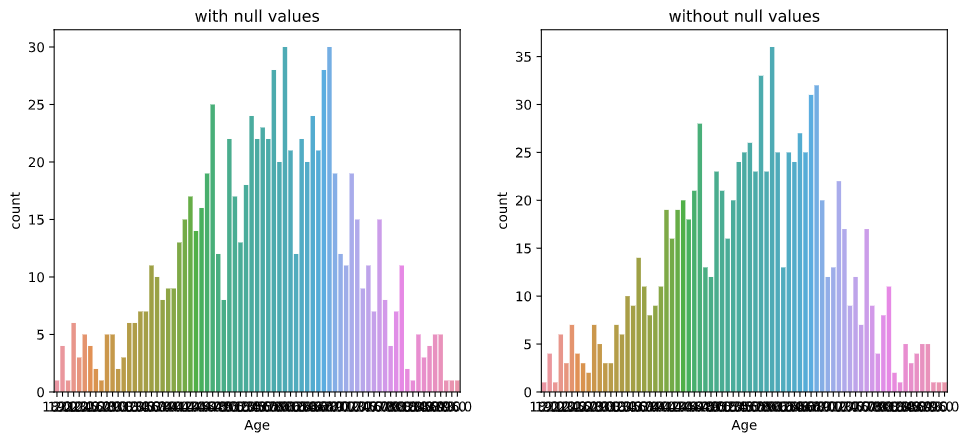
\includegraphics[scale=0.35]{img/age-refill.png}
\end{figure}

Hay que fijarse bien ya que son muchos los valores que puede adoptar la edad, pero vemos cómo no hay ningún valor muy por encima de
lo normal ni que hayan sido \textit{boosteados} en exceso. Con otros valores, como la densidad, también lo podemos hacer, pero
se aprecia un poco menos la diferencia porque hay menos variedad de datos y el 3 destaca sobre todos los demás.
\begin{figure}[H]
    \centering
    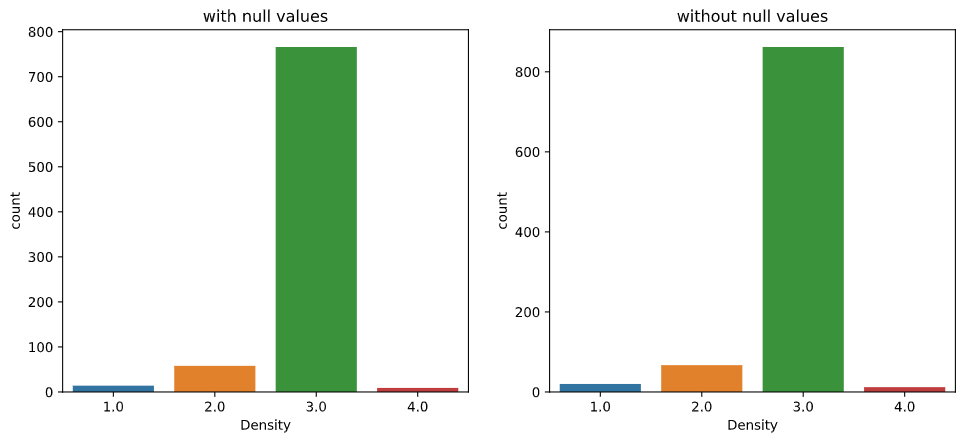
\includegraphics[scale=0.35]{img/density-refill.png}
\end{figure}

Por último, vamos a hacer una media en los atributos que faltan para poder ver también cómo trabaja esta manera de preprocesado.
Podremos observar cómo algunos datos apenas cambian, o es difícil apreciarlo; pero otros, como por ejemplo el valor 3 en 'Margin'
sube bastante, llegando al punto de superar el valor 5 y dándole más importancia en el dataset. No quiere decir que esté mal, ya
que no se sabe cómo serían esos datos en realidad o si pueden venir más datos como estos en un futuro. Pero hay que tener cuidado
porque son datos 'inventados' y, en este caso, originalmente el dataset le da más importancia al 5 que al 3, y lo estamos cambiando.

\begin{figure}[H]
    \centering
    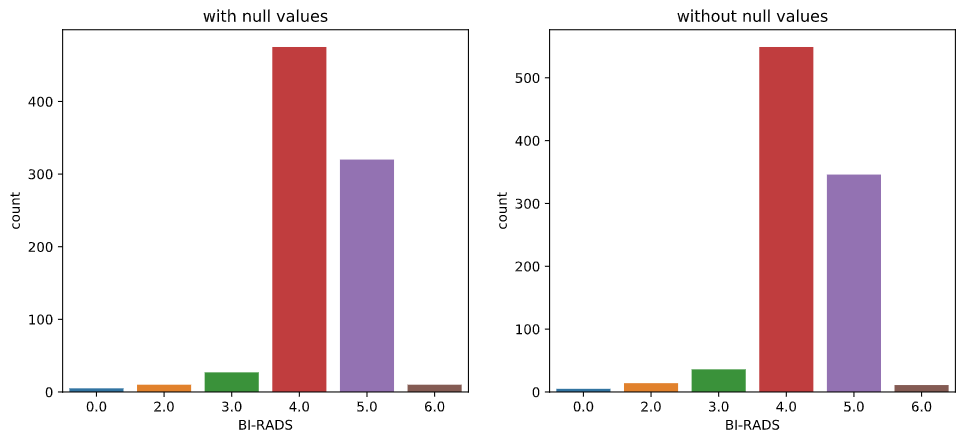
\includegraphics[scale=0.35]{img/birads-refill.png}
\end{figure}

\begin{figure}[H]
    \centering
    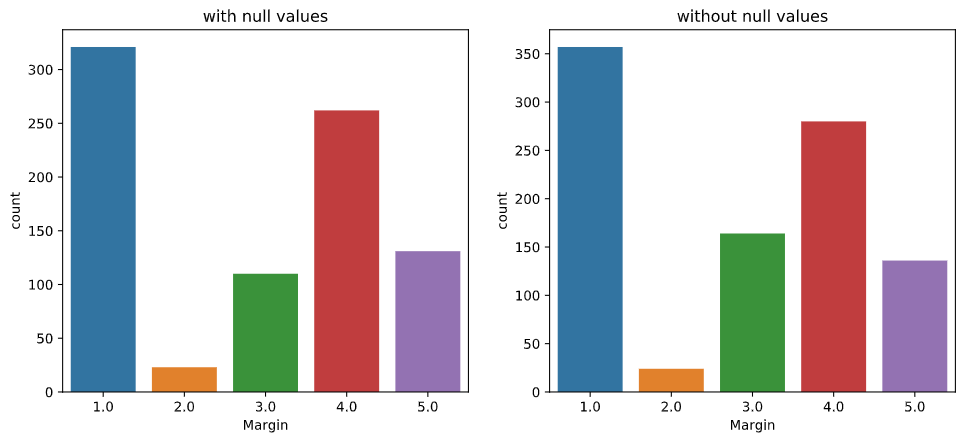
\includegraphics[scale=0.35]{img/margin-refill.png}
\end{figure}


\newpage
\subsection{Gráficas de curva ROC}
No vamos a comentar de nuevo el código, la declaración de los algoritmos, ni la explicación de cómo funcionan, ya que lo hicimos
en la práctica anterior. Únicamente decir que se ha utilizado también un '\textit{Label Encoder}', para los atributos que no son
numéricos, y que se ha hecho la misma división de los datos.

La diferencia con la práctica es que vamos a utilizar simplemente el método \textit{fit()} para entrenar los datos, y después,
con el conjunto de test, hacemos todas las curvas ROC y las mostramos en una sóla gráfica. Este ha sido el resultado:

\begin{figure}[H]
    \centering
    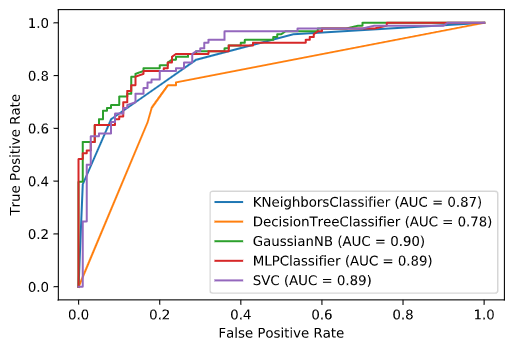
\includegraphics[scale=0.5]{img/curva-roc.png}
\end{figure}

Esta curva representa dos parámetros: tasa de verdaderos positivos y tasa de falsos positivos. El área que hay debajo de la curva
(cálculo de la integral) nos dice cómo es el rendimiento del modelo. Es decir, una curva perfecta subiría hasta la coordenada
$(0,1)$, y su integral daría como resultado 1 (100\% de tasa de verdaderos positivos).


\subsection{Análisis de atributos}
En esta sección realizaremos una serie de representaciones de los distintos atributos para así intentar encontrar alguna relación
entre ellos. Algunos tipos de gráficos ya los hemos utilizado, como puede ser el \textit{countplot}, y el cual lo podemos utilizar
simplemente para saber la cantidad de datos que hay, o la cantidad de benignos y malignos que tenemos:

\begin{figure}[H]
    \centering
    
\includegraphics[scale=0.5]{img/severity-count.png}
\end{figure}

Este gráfico no nos sirve más allá que para contar el número de datos que tiene cada clase, por lo que ya no nos va a servir de
mucho tras haber hecho todo lo anterior. Además de que este tipo de gráfico tampoco nos es útil para relacionar 2 o más categorías.

A continuación, vamos a ver uno llamado \textit{scatterplot}, el cual es un diagrama de dispersión que muestra los datos en forma
de puntos. La posición de cada uno de los puntos viene determinada por un atributo para cada uno de los ejes. Con el diagrama de
dispersión así se podría extraer algún tipo de relación entre los dos atributos, pero para lo que realmente es útil es este tipo
de gráficos en $Seaborn$, es por su capacidad de categorizar los puntos con el atributo objetivo, en nuestro caso la severidad.
Vamos a ver la relación que existe entre la edad y el margen de masa:

\begin{figure}[H]
    \centering
    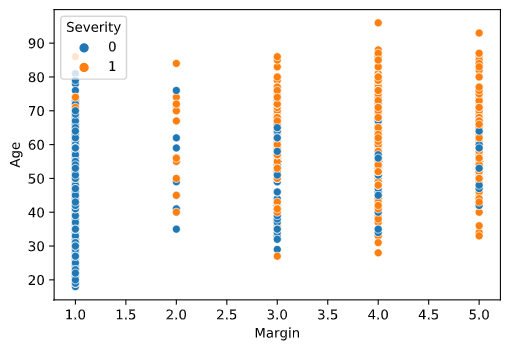
\includegraphics[scale=0.5]{img/scatter-age-margin.png}
\end{figure}

Podemos ver que la relación entre la edad y el margen es prácticamente inexistente, ya que los datos están distribuidos más o menos
de forma equilibrada. No obstante, en cuanto a la severidad, si que podemos ver una clara tendencia a ir hacia la izquierda los
benignos y a la derecha los malignos. Esto quiere decir que cuanto menor sea el margen de masa, más posibilidades hay de que sea
benigno, y viceversa. En cuanto a la edad, lo que vemos no nos dice mucho, ya que hay benignos y malignos repartidos por todas las
edades (es cierto que a edades más bajas vemos un poco más de color naranja y a edades más altas azul, pero nada relevante o para
poder sacar conclusiones).

En la siguiente gráfica, una \textit{boxplot}, vamos a poder observar mejor mejor la diferencia que hemos comentado anteriormente,
porque es un tipo de gráfica (llamada también diagrama de caja) que representa, tanto los cuartiles de los datos con la caja, como
el resto de la distribución con los 'bigotes' que salen de ella.

\begin{figure}[H]
    \centering
    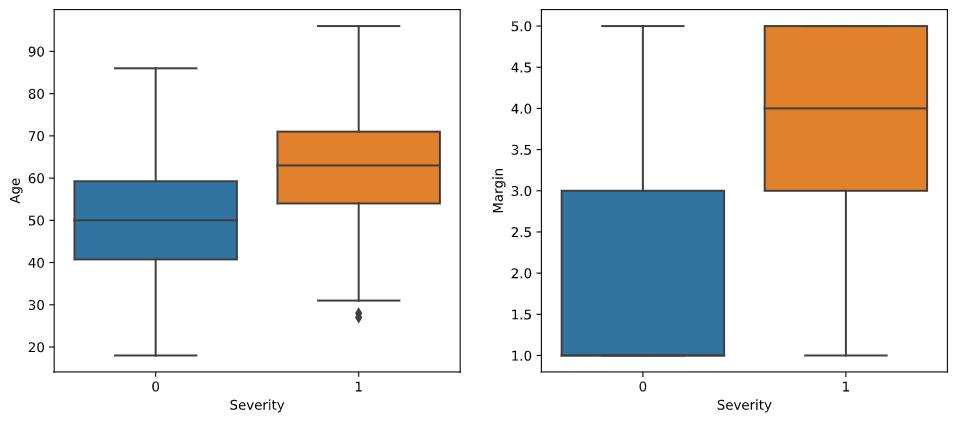
\includegraphics[scale=0.4]{img/boxplot-age-margin.png}
\end{figure}

Ahora vemos más claramente lo anterior

Lo bueno es que elimina valores atípicos


\section{Procesado de datos}




\newpage

% Pagina de bibliografia
\begin{thebibliography}{}
    
    \bibitem{svc}
    Scikit-Learn. \textit{SVC}
    \\\url{https://scikit-learn.org/stable/modules/generated/sklearn.svm.SVC.html#sklearn.svm.SVC}
    
    \bibitem{random_forest}
    Scikit-Learn. \textit{RandomForestClassifier}
    \\\url{https://scikit-learn.org/stable/modules/generated/sklearn.ensemble.RandomForestClassifier.html#sklearn.ensemble.RandomForestClassifier}
    
    \bibitem{neural_network}
    Scikit-Learn. \textit{MLPClassifier}
    \\\url{https://scikit-learn.org/stable/modules/generated/sklearn.neural_network.MLPClassifier.html#sklearn.neural_network.MLPClassifier}
    
    \bibitem{scaler}
    Scikit-Learn. \textit{StandardScaler}
    \\\url{https://scikit-learn.org/stable/modules/generated/sklearn.preprocessing.StandardScaler.html}
    
    \bibitem{pca}
    Scikit-Learn. \textit{PCA}
    \\\url{https://scikit-learn.org/stable/modules/generated/sklearn.decomposition.PCA.html}
    
    \bibitem{bib:learning_curve}
    Scikit-Learn. \textit{plot\_learning\_curve}
    \\\url{https://scikit-learn.org/stable/auto_examples/model_selection/plot_learning_curve.html#sphx-glr-auto-examples-model-selection-plot-learning-curve-py}
    
    \bibitem{bib:recall}
    Scikit-Learn. \textit{recall\_score}
    \\\url{https://scikit-learn.org/stable/modules/generated/sklearn.metrics.recall_score.html}
    
    \bibitem{bib:precision}
    Scikit-Learn. \textit{precision\_score}
    \\\url{https://scikit-learn.org/stable/modules/generated/sklearn.metrics.precision_score.html}
    
    \bibitem{bib:normalize}
    \textit{Should I normalize/standardize/rescale the data?}
    \\\url{http://www.faqs.org/faqs/ai-faq/neural-nets/part2/}
    
    \bibitem{bib:sensitivity-specifity}
    Wikipedia. \textit{Sensitivity and specifity}
    \\\url{https://en.wikipedia.org/wiki/Sensitivity_and_specificity}
    
    \bibitem{bib:svm-kernels}
    DataFlair. \textit{Kernel Functions-Introduction to SVM Kernel \& Examples}
    \\\url{https://data-flair.training/blogs/svm-kernel-functions/}
    
    \bibitem{bib:loss-nn}
    Isaac Changhau. \textit{Loss Functions in Neural Networks}
    \\\url{https://isaacchanghau.github.io/post/loss_functions/}
    
    \bibitem{bib:svm}
    MathWorks\textit{Support Vector Machine}
    \\\url{https://es.mathworks.com/discovery/support-vector-machine.html}
    
    \bibitem{bib:cross_val_score}
    Scikit-Learn. \textit{cross\_val\_score}
    \\\url{https://scikit-learn.org/stable/modules/generated/sklearn.model_selection.cross_val_score.html}
    
    \bibitem{bib:train_test_split}
    Scikit-Learn. \textit{train\_test\_split}
    \\\url{https://scikit-learn.org/stable/modules/generated/sklearn.model_selection.train_test_split.html}
    
    \bibitem{bib:confusion-matrix}
    Scikit-Learn. \textit{Confusion Matrix}
    \\\url{https://scikit-learn.org/stable/auto_examples/model_selection/plot_confusion_matrix.html}
    
    \end{thebibliography}



\end{document}